\chapter{Implementation}

\section{Choice of Language \& Technologies}

The first big implementation decision that was made was the choice of language
that was used to create the system. Before the beginning of term I had made
a proof-of-concept of the system using \emph{C}. I found that the pace of
development was too slow and difficult to make rapid progress. As such
I decided to go in a different direction.

In order to have a shallower learning curve I decided to use a language that
I was familiar with: \emph{Ruby}. I've used Ruby extensively before on many
personal and coursework projects. Besides the experience benefits withe the
language there are other fantastic things about it.

\begin{description}

  \item[Community \& Existing Libraries] \hfill

    There is an extensive preexisting Ruby community that is extremely helpful
    and active. The advantage of this in my case is that there are already many
    libraries for the boilerplate or lower level code that I will be using.
    Importantly it already had bindings for \ac{FUSE} so writing the filesystem
    component of the project could be started immediately.

  \item[Testing Culture] \hfill

    Due to the dynamic nature of the language such as the ability to redefine
    and augment existing classes at runtime it is possible for the programmer
    to create situations where code performs differently based on possible
    hidden factors that have occurred before the execution. This is an
    extremely powerful and useful tool but it must be handled in the correct
    way to eliminate the risk of error. One of the ways that has evolved to
    cope with this is a strong testing culture that is mandated by the
    community for almost all Ruby projects.

    There are numerous libraries that make testing Ruby code quick and easy
    such as \emph{RSpec}. Additionally, large \emph{Ruby} frameworks such as
    \emph{Ruby on Rails} have been developed from the ground up to allow for
    simple and native testing. This culture inspires an Agile attitude to
    refactoring and improving code quality.

  \item[Portability] \hfill

    \emph{Ruby} runs on a number of different operating systems and platforms.
    This factored into my choice as I did not want the available systems that
    the project could run on to be limited by the language. In the end, it was
    \ac{FUSE} (see section \ref{ssec:filesystem}) that was the limiting
    portability factor.

\end{description}

\subsection{Filesystem}
\label{ssec:filesystem}

\ac{FUSE} is often used when creating a filesystem for a custom purpose. It
allows the developer to write code that responds to certain callbacks after it
has been mounted on the existing filesystem at a certain directory. For
example, when a directory is requested \ac{FUSE} will ask the developer's code
what objects are present in that directory by supplying it the argument of
a path. \ac{FUSE} then queries each of these objects to find out if they are
a file or a folder and if there are any permissions that would not allow them
to be shown. These results are then displayed to the user in their file
explorer as if they were actually entities on disk. This has a major advantage
over regular filesystem development which is extremely difficult and requires
extensive knowledge of the kernel to complete.

Other callbacks are provided for the developer to use. The file contents, size,
when files are deleted, or written to are all callbacks that are detected by
\ac{FUSE} and then passed on to the developer's code with the relevant
arguments to the action (e.g. the path being deleted or the text that has been
written to a file).

\subsection{Query GUI}

As discussed above, it isn't simply possible for a query interface to be added
to the filesystem and so a separate but integrated application needed to be
made in order to satisfy this requirement. I elected to use Java and Swing to
complete this task as it is a mature and stable \ac{GUI} toolkit that is
supported on a wide range of operating systems. It is more important that this
application is more portable than the filesystem itself because it would be
feasibly possible to mount the filesystem above over \ac{NFS} and only have
this application on the clients computer to interact with it.

To build the application that allows the user to query the database a GUI
toolkit was needed. Unfortunately \emph{Ruby} is not a suitable language for
this task as it does not have any mature, powerful, and platform-independent
GUI toolkits.

In order to develop this stage I decided to use \emph{Java} and the
\emph{Swing} interface library. This decision was made for two main reasons.

\begin{description}
  \item[Portability] \hfill

    The language that was used for this application must be able to run on any
    platform that the filesystem was used. One of the main advantages of using
    \emph{Java} in any project is that the same code and sometimes even the
    same executable can be run on multiple platforms and systems. This is
    thanks to the ``Write once, run everywhere.'' design
    consideration\footnote{In reality this is more likely to be ``Write once,
    debug everywhere.''}.

  \item[Familiarity] \hfill

    Due to previous projects, jobs, and coursework I am very familiar with the
    \emph{Java} language. Choosing a language that I know well will result in
    better quality code along with a faster development time.

  \item[GUI Toolkit] \hfill

    The \emph{Swing} GUI toolkit for \emph{Java} has its problems (verbosity,
    ugliness). However, even with these problems considered it is still the
    best fit for the application. Selecting \emph{Java} reduced the choices for
    possible interface libraries and due to the fantastic documentation,
    extensibility and customisability then \emph{Swing} was the sensible
    choice.

\end{description}

\section{Development}

\subsection{Filesystem}

The first stage of development was to create the filesystem on which all of the
other projects are based. As mentioned above, over summer I had created
a proof-of-concept system that allowed the user to view a read-only filesystem
representing a database. This was written in \emph{C} and used the native
\emph{FUSE} bindings. Not being satisfied with the development time and
complexities of the language and library I switched to using \emph{Ruby} and
the \emph{FuseFS} library.

The \emph{FuseFS} library works by ``mounting'' a class in a certain directory.
This class is required to implement certain methods (though due to the lack of
type-safety in \emph{Ruby} this can all fall apart at runtime). These methods
are then called when the user interacts with the filesystem whereupon the
return value from the called function is interpreted by the library and shown
in the filesystem. An example of the ``Hello World'' filesystem is shown in
figure~\ref{fig:fusefs}. This filesystem contains a single file called
\texttt{hello.txt} which when read has the contents \texttt{Hello, World!}.

\begin{figure}
\begin{minted}[linenos]{ruby}
class HelloDir
  def contents(path)
    ['hello.txt']
  end

  def file?(path)
    path == '/hello.txt'
  end

  def read_file(path)
    "Hello, World!\n"
  end

  def size(path)
    read_file(path).size
  end
end
\end{minted}
  \caption{A Sample \emph{FuseFS} filesystem.}
  \label{fig:fusefs}
\end{figure}

Using this library I created the filesystem that allowed the user to manipulate
databases. Each table was represented as a directory in the filesystem and
inside were files representing the records in those tables. Each of these were
formatted as \texttt{csv} files for ease of development and portability between
many different spreadsheet editors.

It was noticed that there was no way to select only certain columns to display
in these CSV files rather than just displaying all of them. A new directory was
added inside the table that allowed a user to move columns (represented again
as files) between two folders denoting the used and unused columns. Initially
it was planned that the user would be able to drag the file between the two
directories in order to change this. However, it was found that when using
\ac{FUSE} a file move only looks like a file deletion and a new file write with
no link between them. To overcome this the method which the user changes the
selected columns was changed to use the delete action. This is not ideal and
should be later changed to a more suitable action.

Similar to the \texttt{/proc} filesystem which my project gained much of its
inspiration I added files that could be read to find out information about the
database. For example, this includes the name, list of tables, path, and string
encoding. This allows users to easily find out information by only reading
a file instead of interrogating the database.

\subsubsection{Filesystem DSL Library}

The more I developed this system the slower it became to add new functionality
as the code became more complex. During the Christmas break I decided to write
a new library for creating these filesystem definitions. I decided to start out
with the ``dream library'' by writing down (in \emph{Ruby}) how \emph{I} would
like to build the filesystem. I have included the example I originally wrote in
figure~\ref{fig:skra}. This new \ac{DSL} library is called
\emph{Skra}\footnote{Skr\'{a} is Icelandic for ``file'' or ``directory''.}.

The example below creates a filesystem that is mounted at \texttt{/mount/point}
and contains a directory called \texttt{hello} which has read and write
permissions. Inside this directory are two files: one named \texttt{path} which
contains its own path and the other is called \texttt{time} which when read
will return the current time.

Using this library allowed me to develop the remainder of the project far more
quickly and easily. The library itself was an interesting program to write due
to its implementation as a DSL.

\begin{figure}
\begin{minted}[linenos]{ruby}
Filesystem.new "/mount/point" do
  directory "hello", :perms => [:r, :w] do
    file "path" do |path|
      # File contains its own path.
      path
    end

    file "time" do |path|
      # Shows the current time.
      Time.now.to_s
    end
  end
end
\end{minted}
  \caption{An example \emph{Skra} layout.}
  \label{fig:skra}
\end{figure}

\subsection{Query Language}

You may have noticed above that I have not mentioned how the database is
queried. This is due to the query problem that was mentioned earlier in
section~\ref{sec:queryproblem}. The solution which was decided on above was to
create a two-tiered system for querying. Firstly, a language is created that
allows even complex queries to be written sequentially and out of order. This
allows more advanced users to use this directly when querying. Secondly, an
application is created that allows users who are not familiar with databases to
invisibly create this language before using the same process as the more
advanced users to query the database. This section deals with the creation of
this intermediate language.

At the time this was planned to only be a very small part of a larger project
and as such spending a large portion of time creating a whole new language with
its own grammar, parser, and semantics was not a wise time investment. In order
to gain all of these language building blocks for ``free'' \emph{Ruby} was
again used. The \emph{Ruby} language has often been used as the base of other
\acp{DSL} such as the build tool
\emph{Rake}\footnote{http://rake.rubyforge.org/} or the testing framework
\emph{RSpec}\footnote{http://rspec.info/}. Both of these tools have a syntax
that while being completely executable is able to be expressive and simple.

Using this same trait of \emph{Ruby} in the \ac{DSL} allowed the creation of
a query language that did not resemble its parent language while using it as
a strong foundation. By using \emph{Ruby} the fantastic library \emph{ARel}
library\footnote{\url{https://github.com/rails/arel}} could also be used in
order to generate the \ac{SQL} from relational algebra. \emph{ARel} is
a powerful and mature piece of software (it powers the \ac{ORM} in the popular
web framework \emph{Ruby on Rails}). However, it is not designed to be directly
used in the manner required for this project and as such additional changes
were required in order to make it suitable for the \ac{DSL}.

Various additions were made to allow for a clean interface between the two
sides of the system. New functions that improved the ease-of-use and script
like qualities of the language were added (e.g. The \texttt{Table} function
which removed the ugly overhead required to define a new table for use in
\emph{ARel}). A command line interface was added to the system to complete its
functionality. The entire system was named \emph{Squeal} as it was a Pig Latin
for \ac{SQL}. An example query is shown in figure~\ref{fig:squeal}.

\begin{figure}
\begin{minted}[linenos]{ruby}
users = Table :users
grades = Table :grades

# Define predicates separately
predicate = users[:name].eq("Chris Brown")

# Simply Sequential
user_grades = join(users, grades, :id, :user_id)
user_where = where(user_grades, predicate)
user_window = limit(user_where, 1)

# Useful Chaining
user_order = user_window.order(grades[:mark])

Output select(user_grades, grades[:course], grades[:mark])
\end{minted}
  \caption{A Squeal script for finding the course and mark for the lowest
  grade on record.}
  \label{fig:squeal}
\end{figure}

\subsection{Query GUI}

In order to generate this language a \ac{GUI} needs to be created that allows
users to draw the graph representation of their query. This program can then be
used by users of all experience levels. The advantage of using relational
algebra for our intermediate language is that is is composeable and therefore
a graph based interface can be used to create these queries.

As discussed above, \emph{Swing} and \emph{Java} were used in order to create
the interface. The most challenging component of this was creating a new user
interface element for the graph. This component was completely custom and it
was built with reuse in mind. This component can be embedded in other
applications if the developer wishes for a pre-built solution for building
these queries.

The user interface is extremely minimal. The only significant element in the
window is the graph creation component mentioned above. All of the user
interaction with the program is done by using the right-click menu of this
component. When a user has finished creating their query they are able to
easily save this file to the filesystem where it is executed.

The operation of the program is relatively simple. Users right click on the
canvas and place nodes corresponding to the different operators that can be
performed by the query. After a node is placed the user is prompted to enter
the attributes of the node (such as the number of records to limit or the
predicate of a filter node). The user is then able to drag connectors between
these nodes in order to create the final query.

An example of a query is shown in figure~\ref{fig:bacon}. This would generate
the Squeal script that was shown before in figure~\ref{fig:squeal}.

\begin{figure}
  \centering
  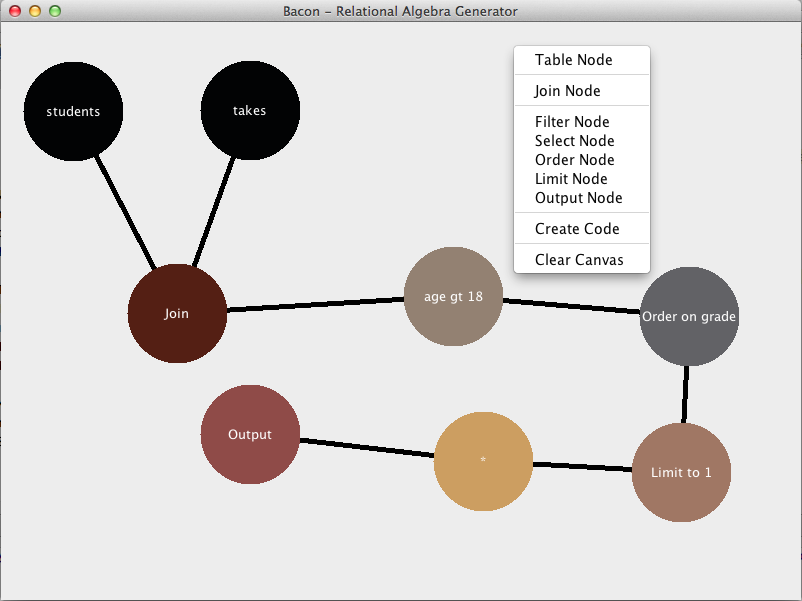
\includegraphics[width=0.9\textwidth]{images/bacon}
  \caption{Example GUI Query}
  \label{fig:bacon}
\end{figure}
